% \documentclass[runningheads,anonymous]{llncs} 
\documentclass[runningheads]{llncs} 
% \documentclass[sigconf,natbib=false,anonymous,nonacm]{acmart}

\usepackage{amsmath} % text in equation 
\usepackage{amsfonts}  
\usepackage{setspace} % setstretch
\usepackage{graphicx} % resizebox
\usepackage{makecell} % for makecell
\usepackage{mathtools} % for \begin{multlined}
% \usepackage{algorithm}
% \usepackage{algpseudocode}
\usepackage{enumitem}
\usepackage[linesnumbered,ruled,noend]{algorithm2e}
\usepackage[misc]{ifsym}

\usepackage{caption} % for subfigure error
\usepackage{subcaption} % for subfigure error
\usepackage{mathtools} % for ceil
\usepackage{hyperref}
\usepackage{nameref}
\usepackage{xcolor}

\usepackage[maxnames=1, giveninits=true, doi=false, isbn=false, url=false]{biblatex}
% maxnames=2:限制作者人数,超过则用 “et al.” 表示。
% giveninits=true:将名字缩写为首字母。
% doi=false, isbn=false, url=false:禁用不需要的信息(如 DOI、ISBN 和 URL)。

\usepackage{tikz}
\usetikzlibrary{positioning}

\newcommand{\tablefolder}{tab} % Define a macro to hold the path
\newcommand{\inull}[1]{}
%\newcommand{\kdpbat}{$k$-DP$_{bat}$}

%%
%% \BibTeX command to typeset BibTeX logo in the docs
\AtBeginDocument{%
  \providecommand\BibTeX{{%
    Bib\TeX}}}

%% Declare bibliography sources (one \addbibresource command per source)
\addbibresource{main.bib}

% from https://muc2022.mensch-und-computer.de/en/cfp-en/guidelines-for-publication/
% \settopmatter{printacmref=false, printccs=false}
% \setcopyright{none}

\makeatletter
% \@printcopyrightfalse
% \@printpermissionfalse
% \@acmownedfalse
\makeatother



\begin{document}
% \pagestyle{empty} % 排除页码
\pagenumbering{gobble} % 排除页码
\newcommand{\iG}{\mathcal{G}}
\newcommand{\iV}{\mathcal{V}}
\newcommand{\iE}{\mathcal{E}}

\title{\texttt{ShareDP}: Finding k Disjoint Paths for Multiple Vertex Pairs}

% example
% \author{First Author\inst{1} \and
% Second Author\inst{2,3} \and
% Third Author\inst{3}}
% \authorrunning{F. Author et al.}
% \institute{
% xxx\\
% \email{lncs@springer.com}\and
% xxx\\
% \email{lncs@springer.com}\and
% xxx\\
% \email{lncs@springer.com}
% }             

\author{Zhiqiu Yuan\inst{1} \and
Youhuan Li\inst{2} \and
Lei Zou \Letter\inst{1} \and
Linglin Yang\inst{1}}
\authorrunning{Z. Yuan et al.}
\institute{
Peking University\\
\email{\{yuanzhiqiu, linglinyang\}@stu.pku.edu.cn, zoulei@pku.edu.cn} \and
Hunan University\\
\email{liyouhuan@hnu.edu.cn}
}
% \institute{
% Peking University\\
% \email{yuanzhiqiu@stu.pku.edu.cn} \and
% Hunan University\\
% \email{liyouhuan@hnu.edu.cn} \and
% Peking University\\
% \email{zoulei@pku.edu.cn} \and
% Peking University\\
% \email{linglinyang@stu.pku.edu.cn}
% }
% \maketitle              

%%
%% The "author" command and its associated commands are used to define the authors and their affiliations.
% \author{Youhuan Li}
% \affiliation{%
%  \institution{Hunan University}
% %  \streetaddress{P.O. Box 1212}
% %  \postcode{43017-6221}
% }
% \email{liyouhuan@hnu.edu.cn}

% \author{Lei Zou} %$^\dagger$
% \affiliation{%
%  \institution{Peking University}
% }
% \email{zoulei@pku.edu.cn}
% \authornote{Lei Zou is the corresponding author.}

% \linepenalty=1000
% \captionsetup[table]{skip=5pt}
\maketitle 
% \vspace{-15pt}
\begin{abstract}
Retrieval-Augmented Generation (RAG) is often used with Large Language Models (LLMs) to infuse domain knowledge or user-specific information. In RAG, given a user query, a retriever extracts chunks of relevant text from a knowledge base. These chunks are sent to an LLM as part of the input prompt. Typically, any given chunk is repeatedly retrieved across user questions. However, currently, for every question, attention-layers in LLMs fully compute the key values (KVs) repeatedly for the input chunks, as state-of-the-art methods cannot reuse KV-caches when chunks appear at arbitrary locations with arbitrary contexts. Naive reuse leads to output quality degradation.  This leads to potentially redundant computations on expensive GPUs and increases latency. In this work, we propose \sys, a system for managing and reusing precomputed KVs corresponding to the text chunks (we call \textit{chunk-caches}) in RAG-based systems. We present how to identify \hl{\textit{chunk-caches} that are reusable}, how to efficiently perform a small fraction of recomputation to \textit{fix} the cache to maintain output quality, and how to efficiently store and evict \textit{chunk-caches} in the hardware for maximizing reuse while masking any overheads. With real production workloads as well as synthetic datasets, we show that \sys reduces redundant computation by \textbf{51\%} over SOTA prefix-caching and \textbf{75\%} over full recomputation.
\hl{Additionally, with continuous batching on a real production workload, we get a \textbf{1.6$\times$} speedup in throughput and a \textbf{2$\times$} reduction in end-to-end response latency over prefix-caching while maintaining quality, for both the \llama-3-8B and \llama-3-70B models. 
}
\end{abstract}





\documentclass[../main.tex]{subfiles}
\graphicspath{{../images/}}
\makeatletter
\def\input@path{{../images/}}
\makeatother
\begin{document}
\section{Introduction}
\begin{figure}
\centering
\begin{tikzpicture}
\node[inner sep=0pt] (ws) at (0, 0) {
\includegraphics[height=.4\textwidth, trim={10cm 0 10cm 0},clip]{world_space.png}};
\node[inner sep=0pt] (cs) at (6,0) {\includegraphics[height=.4\textwidth, trim={10cm 1cm 10cm 4cm},clip]{conf_space.png}};
\end{tikzpicture}
\vspace{-5pt}
\label{fig:pbrm_intro}
\caption{\textbf{Left}: Shows world space obstacles as grey spheres. Robots start and goal configuration is colored red and green, respectively. Configurations along the computed path are colored transparent blue. \textbf{Right:} Mapped world space scenario to configuration space. Obstacle region is the grey mesh. Red spheres are collision-free regions computed by the neural SCDF. The optimized shortest path in the convex corridor is the blue curve.}
\vspace{-25pt}
\end{figure}
Motion planning is the problem of finding a collision-free trajectory that connects a given start and goal configuration. The planning takes place in the configuration space of the robot. For single body robots, like mobile robots or drones, the configuration space and the world space are usually the same. This simplifies the planning, since explicit obstacle representations are available which enables geometrical tools like separating hyperplanes, smallest distance to obstacles etc., to be used when designing motion planning algorithms. For multi-body robots like manipulators, the situation is completely different. The world space obstacles are usually mapped to non-convex regions, and to make the problem even harder, the mapping is usually not known. Forming explicit representations of the obstacle region in the configuration space is usually too expensive or intractable. Despite all of this, sampling based planners are used with great success, which mainly is due to their use of implicit representations of the obstacle region. The basic idea is to construct a graph in the configuration space that covers and connects the collision-free region. From this graph, a path can be extracted that connects a given start and goal configuration. The approach is computationally expensive, since the graph is constructed with the smallest geometrical building block available, points, which represents a collision-check. Furthermore, the extracted paths from the graph are non-smooth and jagged due to the stochastic nature of the approach. This adds an additional post-processing step to the process, where the paths are shortcutted and smoothened, before the path can be used for tracking. Clearly a lot of time is invested to form this graph and produce smooth paths. Thus, if the obstacles start to move, then all of this work is done in no use, since all points that make up this graph need to be re-verified, which is simply too time consuming to be done in real time.
\\\\
In this work, we want to address the existing drawbacks of the sampling based planners. Our main contribution is an improved motion planner where each vertex in the graph covers a collision-free region in the form of a sphere instead of a point and where the edges are formed with neighboring intersecting spheres. This representation has the advantage of instead of returning piecewise linear paths, returning a sequence of overlapping spheres, i.e. a convex corridor, that connects a given start and goal configuration, illustrated in Figure \ref{fig:pbrm_intro}. This convex corridor allows us to use convex optimization to produce smooth trajectories, instead of computationally expensive post-processing methods. The representation further allows us to estimate the coverage of the collision-free space, which gives us awareness and feedback in the offline roadmap construction phase. Finally, our representation is simple to adapt to moving obstacles, simply requery for the new radii and recheck for intersections. 
\\\\
The spherical collision-free regions are formed using a signed distance function (SDF), which is a function that returns the smallest distance from an arbitrary point to the boundary of an obstacle. As the name implies, the distance is signed, thus if the point is inside the obstacle it is negative otherwise positive. If the distance is positive, a sphere with radius equal to the distance is guaranteed to cover a collision-free region. Using an SDF in motion planning is not new, but what is novel about our approach is that we express the distance in the configuration space instead of the world space and by doing so allows us to form these convex collision-free regions. We refer to the resulting SDF as a signed configuration distance function (SCDF). Computing an SCDF analytically is non-trivial, our approach is therefore to parameterize the SCDF with a deep neural network and learn the mapping by supervised learning. Our resulting neural SCDF can compute distances for different parameter values of obstacle shapes and we also show how multiple distances can be combined, thus making our approach flexible.
\section{Related work}
Motion planning algorithms can roughly be divided into three families, grid-based, sampling based and optimization based methods. Grid-based methods (GBM) discretize the planning space from which a graph is then compiled. A standard search method is A$^\star$ \citep{a_star}, which is classified as an \textit{informed} search method, since it employs a heuristic function to speed up the search. A$^\star$ guarantees to return an optimal path at the level of discretization used. GBMs usually discretize the planning space by a regular lattice and this limits the GBMs to problems with low dimensionality due to the curse of dimensionality. Thus, GBMs are usually limited to single-body robots where the degrees of freedom (DOF) are low. To overcome the inherent scaling problem with the GBMs, stochastic methods are usually used for multi-body robots. These methods are termed as sampling-based methods (SBM) and core members within this family are the rapidly-exploring random trees (RRT) \citep{rrt} and the probabilistic roadmap (PRM) \citep{prm}. RRT grows a tree from the start configuration and explores the collision-free region in a rapid way until it is able to connect to the goal region. RRT is usually improved by bi-directional planning \citep{rrt_connect}, i.e. an additional tree is grown from the goal configuration and the trees are tested for connection after any tree has been expanded. RRT is a single-query method, thus it searches for a path from scratch each time it is queried. Contrary to this, PRM is a multi-query method, which solves for multiple queries without starting from scratch. PRM does this by creating a roadmap (graph) that covers the collision-free space as an offline step. The graph is then used to solve for multiple queries. PRMs are used in cases where the environment does not change since the extra offline step is too computationally costly and needs to be re-done if the environment is changed. In our work, we address this inherent issue by using a different roadmap representation. Our vertices in the graph cover a collision-free region in the form of spheres and we form the edges by checking for intersecting spheres. If something in the environment changes, we recompute the spheres radii and recheck the intersections, without relying on collision detection. We use a trained neural network to compute the sphere radius, therefore querying for the radius can be done fast, hence our representation enables the PRM for dynamic environments.
\\\\
In the recent decades, optimization based methods (OBM) \citep{chomp, schulman, itomp, stomp} have been introduced as an alternative to SBM for multi-body robots. Like the SBM, the OBMs scale well to higher dimensional problems and produce smoother motion. It is common to use a SDF in the optimization since it is a smooth function, thus enabling gradient-based methods. However, the standard way of expressing the SDF is in world space. The distance therefore needs to be mapped to the configuration space by the forward kinematics. This mapping makes the optimization problem a non-linear program (NLP), which is computationally expensive to solve. Recently, a different approach has been proposed. In \cite{mp_gcs} motion planning is formulated as a convex optimization problem by using the graph of convex sets framework \citep{gcs}. The underlying idea is to decompose the collision-free space into intersecting convex sets from which a convex optimization problem is formulated. In cases where an explicit representation of the obstacles in the configuration space exists, like for single-body robots, creating collision-free convex regions can be done fast \citep{iris}. For multi-body robots, this is non-trivial. Existing work does this successfully \citep{iris_nlp, iris_c} by an optimization based approach, but the methods are still too time consuming to be used in the presence of moving obstacles. Our approach is instead to use deep learning to learn an SDF expressed in the configuration space. With this, we can query for shortest distances to the collision boundary, which allows us to expand spherical regions which are collision-free. Our approach is fast and therefore enables our suggested roadmap planner to be used in dynamic environments.
\\\\
Recent research has focused on learning collision detection \citep{fk_kernel_distance, diffco, graphdistnet} by predicting the signed distance between the robot links and the surrounding obstacles in the world space. The learned SDF is used in trajectory optimization but since the distance is expressed in the world space, the problem becomes an NLP and therefore takes a long time to solve. We take a novel approach and suggest to instead express the signed distance in the configuration space. This allows us to improve the PRM at the same time as it enables convex optimization for trajectory optimization, which runs faster and is more reliable than NLP solvers. In \cite{cspf} a learned signed distance function in the configuration space is proposed similar to our approach. However, their approach is restricted to point cloud representations, while we propose to represent the obstacles as parameterized geometric shapes, e.g. spheres. Furthermore, we also show how to use our learned SCDF to improve an existing roadmap planner.
\section{Problem formulation}
A robot is located in the world space, $\W \subset \R^3 $. The unique location of the robot is given by its configuration $\q \in \C$, where $\C$ is the configuration space. The set of points covered by the robots bodies at a certain configuration is expressed as $\B(\q) \subset \W$. The robot is surrounded by $\NrObst$ obstacles $\O = \bigcup_{i=1}^{\NrObst} \O_i$, where  $\O_i \subset \W$. The representation of the obstacle in the configuration space is the set $\C\O_i = \{\q \in \C \: |\: \B(\q) \cap \O_i \neq \emptyset \}$. The obstacle space is formed as $\Co = \bigcup_{i=1}^{\NrObst} \C \O_i$. The complement is referred to as the free space, $\Cf = \C \setminus \Co$. The path planning problem is a tuple, ($\Cf$, $\qStart$, $\qGoal$), where we want to connect a query pair, consisting of a start, $\qStart$, and goal configuration, $\qGoal$, with a geometric path, $\q(s): [0, 1] \mapsto \Cf$, such that $\q(0)=\qStart$ and $\q(1)=\qGoal$, or report correctly when such a path does not exist.
\end{document}

\section{Adaptive labeling as a Markov decision process} 
\label{sec:formulation}

We illustrate our formulation for model evaluation, and extend it to the ATE estimation setting at the end of the section. 
Our goal is to evaluate the performance of a prediction model $\model: \statdomain \to \mathcal \labeldomain$ over the input distribution $P_X$ that we expect to see during deployment.  Given inputs $X  \in \mc{X}$,   labels/outcomes are generated
 from some unknown function $f\opt$: $
      Y = f\opt(X) + \varepsilon$, where $\varepsilon$ is the noise.
      %~~~\mbox{where}~~\varepsilon \sim N(0, \sigma^2)
  % \begin{equation*}
  %     Y = f\opt(X) + \varepsilon~~~\mbox{where}~~\varepsilon \sim N(0, \sigma^2).
  % \end{equation*}
When ground truth outcomes are costly to obtain, previously collected labeled data $\mc{D}^0 := \{(X_i,Y_i)\}_{i \in \mc{I}}$ 
typically suffers selection bias and covers only a subset of the support of input distribution $P_X$ over which we aim to evaluate the model performance. 

Assuming we have a   pool of data $\xpool$, we design
 adaptive sampling algorithms that iteratively select
inputs in $\xpool$ to be labeled.
Since labeling inputs takes time in practice, we model
real-world instances by considering \emph{batched} settings. Our goal is to sequentially label batches of data to accurately estimate model performance over $P_X$ and therefore we assume we have access to a set of inputs $\xeval \sim P_X$. %We assume the modeler pays a fixed and equal cost for each label/outcome. 
%Our framework is general as we do not assume \xpool∼PX\xpool \sim P_X.
We use the squared loss to illustrate our framework,
where our goal is to evaluate $\E_{X \sim P_X}[ (Y - \model(X))^2]$. Under the ``likelihood" function $p(y | f, x) = p_{\varepsilon}(y - f(x))$,  let $g(f)$ be the performance of the AI model $\model(\cdot)$ under the  data generating function $f$, which we refer to as our estimand of interest.
When we consider the mean squared loss,  $g(f)$ is given by 
\begin{align}
    g(f) \defeq \E_{X \sim P_X}\left[ \E_{Y \sim p(\cdot|f,X) } \Big[ (Y - \model(X))^2 \Big] \mid f \right]. \label{eqn:l2-g-f}
\end{align}
Our framework is general and can be extended to other settings. For example, a clinically useful  metric is \texttt{Recall}, defined as the fraction of individuals that the model $\model(\cdot)$ correctly labels as positive  among all the individuals who actually have the positive label 
\begin{align*}
    g(f) \defeq  \E_{X \sim P_X}\left[ \E_{Y \sim p(\cdot|f,X) } \Big[\indic{\model(X)>0}|Y=1\Big] \mid f\right].
\end{align*}
 
  Since the true function $f\opt$ is unknown, we  model it from a Bayesian perspective by formulating a posterior given the available supervised data. We refer to uncertainty over the data generating function $f$ as \emph{epistemic} uncertainty---since we can resolve it with more data---and that over
 the measurement noise $\varepsilon$ as \emph{aleatoric} uncertainty. 
Assuming independence given features $X$, we model the  likelihood of the data via the product 
$p({Y}_{1:m}|f, {X}_{1:m}) = \prod_{i=1}^m p(Y_i|f,X_i)$.
 Our prior belief  $\mu$ over functions $f$   reflects our uncertainty about how
labels are generated given features. 
To adaptively label inputs from $\mc{X}_{\rm pool}$, we assume access to an uncertainty quantification (UQ) method that provides posterior beliefs $\mu(f \mid \mc{D})$ given
any supervised data $\mc{D}:= \{(X_i,Y_i)\}_{i \in \mc{I}}$. As we detail  in Section~\ref{sec:uq}, our framework can leverage both classical 
Bayesian models like Gaussian processes and recent advancements in deep learning-based UQ  methods.

As new batches are labeled, we update our posterior beliefs about $f$ over time, which we view as ``state transitions'' of a dynamical system.
Recalling the Markov decision process depicted in Figure~\ref{fig:overview}, we sequentially label a batch of inputs from $\mc{X}_{\rm pool}$ (actions), which lead to state transitions (posterior updates).
Specifically, our initial state is given by $\mu_0(\cdot) = \mu(\cdot \mid \mc{D}^0)$, where $\mc{D}^0$ represents the initial labeled dataset.
At each period $t$, we label a batch of $K_t$ inputs $\mc{X}^{t+1} \subset \mc{X}_{\rm pool}$ resulting in labeled data $ \mc{D}^{t+1} = (\mc{X}^{t+1}, \datay^{t+1})$. After acquiring the labels at each step $t$, we update the posterior state to $\mu_{t+1}(\cdot) = \mu_t(\cdot \mid \mc{D}^{t+1})$. Modeling practical instances, we consider a small horizon problem with limited adaptivity $T$. Formulating an MDP over posterior states has long conceptual roots, dating back to the Gittin's index for multi-armed bandits~\citep{Gittins79}.

 We denote by $\pi_t$ the adaptive labeling policy at period $t$. We account for randomized policies $\datax^{t+1} \sim \pi_t(\mu_t)$ with a flexible batch size $|\datax^{t+1}| = \batchsize_t$.   
We assume $\pi_t$ is $\mc{F}_t-$measurable for all $t < T$, where $\mc{F}_t$ is the filtration generated by the observations up to the end of step $t$.
 Observe that $\mu_{t+1}$ contains randomness in the policy $\pi_t$ as well as randomness in $\datay^{t+1} \mid (\datax^{t+1},\mu_t)$. Letting $\pi = \set{\pi_0,....,\pi_{T-1}}$,  we minimize the uncertainty over $g(f)$
 at the end of data collection
\begin{align}
H(\pi) \defeq \E_{\mc{D}^{1:T} \sim \pi} \left[G(\mu_{T}) \right]  \defeq  \E_{\mc{D}^{1:T} \sim \pi} \left[G(\mu(\cdot \mid \mc{D}^{0:T})) \right]
%\defeq \E_{\mc{D}^{1:T} \sim \pi} \left[ \V_{f \sim \mu_{T}}  g(f)  \right]
     = \E_{\mc{D}^{1:T} \sim \pi} \left[ \V_{f \sim \mu(\cdot \mid \mc{D}^{0:T})}  g(f)  \right],
     \label{eqn:general-obj}
\end{align}   
where $G(\mu_T) = \V_{f \sim \mu_T}  g(f)$.
In the above objective~\eqref{eqn:general-obj}, we assume
that the modeler pays a fixed and equal cost for each outcome. 
Our framework can also seamlessly accommodate variable labeling cost. Specifically, we can define a cost function $c(\cdot)$ 
 applied on the selected subsets 
 and update the objective~\eqref{eqn:general-obj} accordingly to include the term  $\lambda c(\mc{D}^{1:T})$,
 where $\lambda$
 is the penalty factor that controls the trade-off between minimizing variance and cost of acquiring samples.


Our framework can be easily extended to causal estimation problems.  Consider a feature vector ${X}$ and suppose we have two treatment arms $Z \in \{0,1\}$. Our objective is to evaluate the average treatment effect over the population distribution $P_X$.  Given feature vector $X$, and treatment $Z$,  outcomes are generated from an unknown function $f\opt$: 
$Y = f\opt(X,Z) + \varepsilon.$
%~~~\mbox{where}~~\varepsilon \sim N(0, \sigma^2)
  % \begin{equation*}
  %     Y = f\opt(X) + \varepsilon~~~\mbox{where}~~\varepsilon \sim N(0, \sigma^2).
  % \end{equation*}
The available data is denoted by $\mc{D}^0 := \{X_i,Y_i,Z_i\}_{i \in \mc{I}}$ and given a pool of candidates 
$\xpool$, we want an
 adaptive sampling algorithms that iteratively select
candidates in $\xpool$ to be assigned a random treatment so that we can estimate average treatment effect efficiently. Under the ``likelihood" function $p(y | f, x, z) = p_{\varepsilon}(y - f(x,z))$,  let $g(f)$ represent  the average treatment effect, which is our estimand of interest. Formally, this is expressed as:
\begin{align}
g(f) \defeq \E_{X \sim P_X} \left[\E_{Y_1 \sim p(\cdot|f,X,Z=1) , Y_0 \sim p(\cdot|f,X,Z=0)} \left[Y_1 -  Y_0 \right]\mid f \right]. \label{eqn:ate-g-f}
\end{align}




 %Again the true function $f\opt$ is unknown and we model it from a Bayesian perspective by formulating a posterior  given available data.
 Our prior belief  $\mu$ over functions $f$, now 
 reflects our uncertainty about how
outcomes are generated given features and treatments. 
  We sequentially observe outcome of a batch of inputs from $\mc{X}_{\rm pool}$ (actions), and treatments assigned to this batch. We assume that selected batch of inputs $\mc{X}^t$ is randomly assigned treatments $\mc{Z}^t$ with each $Z\sim p_Z$. We summarize our formulation in Figure~\ref{fig:MDP_framework_flowchart}.
%Specifically, our initial state is given by $\mu_0(\cdot) = \mu(\cdot \mid \mc{D}^0)$ and at each period $t$, we get outcomes for a batch of $K$ candidates $\mc{X}^{t+1} \subset \mc{X}_{\rm pool}$, with randomly assigned treatments $\mc{Z}^{t+1}$ (with each $Z\sim p_Z$) and get the data $ \mc{D}^{t+1} = (\mc{X}^{t+1} \times \datay^{t+1} \times \mc{Z}^{t+1} )$. After acquiring the data at each step $t$ we update posterior state to $\mu_{t+1}(\cdot) = \mu_t(\cdot \mid \mc{D}^{t+1})$. Modeling practical instances, we consider a small horizon problem with limited adaptivity $T$.  We denote by $\pi_t$ the adaptive labeling policy at period $t$. We account for randomized policies $\datax^{t+1} \sim \pi_t(\mu_t)$ with a flexible batch size $|\datax^{t+1}| = \batchsize_t$.   
Again, we assume $\mu_t$ is $\mc{F}_t-$measurable for all $t < T$, where $\mc{F}_t$ is the filtration generated by the observations up to the end of step $t$.
 Observe that $\mu_{t+1}$ contains randomness in the policy $\pi_t$, randomness in treatment assignment $\mc{Z}^{t+1}$ and randomness in $\datay^{t+1} \mid (\datax^{t+1}, \mc{Z}^{t+1},\mu_t)$. Letting $\pi = \set{\pi_0,....,\pi_{T-1}}$,  we minimize the uncertainty over $g(f)$
 at the end of data collection:
\begin{align}
\E_{\mc{D}^{1:T} \sim \pi} \left[G(\mu_{T}) \right] \defeq
\E_{\mc{D}^{1:T} \sim \pi} \left[ \V_{f \sim \mu_{T}}  g(f)  \right]
= \E_{\mc{D}^{1:T} \sim \pi} \left[ \V_{f \sim \mu(\cdot \mid \mc{D}^{0:T})}  g(f)  \right].
\label{eqn:general-ate-obj}
\end{align}  


 

\begin{figure}[ht]
\centering
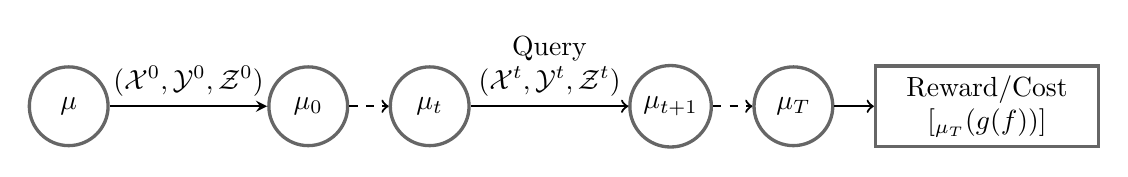
\begin{tikzpicture}
[
roundnode/.style={circle, draw=black!60, very thick, minimum size=10mm},
squarednode/.style={rectangle, draw=black!60, very thick, minimum size=10mm, align =center,text width = 26mm},
]
%Nodes
\node[roundnode]      (maintopic)                              {$\mu$};
\node[roundnode]        (circle1)       [right=20mm of maintopic] {$\mu_0$};
\node[roundnode]      (circle2)       [right=5mm of circle1] {$\mu_t$};
\node[roundnode]        (circle3)       [right=20mm of circle2] {$\mu_{t+1}$};
\node[roundnode]        (circle4)       [right=5mm of circle3] {$\mu_T$};
\node[squarednode]        (circle5)       [right=5mm of circle4] {Reward/Cost $\E \left[ \V_{\mu_T} (g(f))\right]$};


%Lines
\draw[thick, ->, >=stealth] (maintopic.east) -- node[anchor=south] {$(\mathcal{X}^0,\mathcal{Y}^0,\mathcal{Z}^0)$} (circle1.west);
\draw[thick, ->, dashed] (circle1.east) --  (circle2.west);
\draw[thick, ->] (circle2.east)  -- node[above, align =center, text width = 18mm] { Query $(\mathcal{X}^t,\mathcal{Y}^t,\mathcal{Z}^t)$} (circle3.west);
\draw[thick, ->,dashed] (circle3.east) --  (circle4.west);
\draw[thick, ->] (circle4.east) --  (circle5.west);


\end{tikzpicture}
\caption{MDP framework for adaptive labeling to efficiently estimate the average treatment effect (ATE).}
\label{fig:MDP_framework_flowchart}
\end{figure}
 









\begin{comment}
\subsection{Broader applicability of the framework to other problem settings} \label{sec:broad-framework-accuracy}
 

Although  we describe our setting in a healthcare setting with the objective  to estimate the recall of a trained AI model $\model(\cdot)$, the framework caters to many other problem settings. The extension to the evaluation of model based on accuracy (in regression setting) is straightforward, we simply replace the definition of recall $g(f)$ in~\eqref{eqn:l2-g-f} with
\begin{align*}
    g(f) = \E_{\substack{ y \sim p(y|f,x) \\  \forall x \in \mathcal X}} \big( \E_{{\textbf x} \sim p_x} [y-\model(x)]^2 \big).
\end{align*}


\textcolor{red}{To discuss if we need to have it here}
We can also extend this setting to the efficient estimation of the ATE as well. We describe these in detail below:

\begin{itemize}
    
    \item Estimating accuracy:  \[g(f) = \E_{\substack{ y \sim p(y|f,x) \\  \forall x \in \mathcal X}} \big( \E_{{\textbf x} \sim p_x} [y-\model(x)]^2 \big)\]
%    \item Estimating ATE with known control arm: 
%\[g(f) = \E_{\substack{ y \sim p(y|f,x) \\  \forall x \in \mathcal X}} \big( \E_{{\textbf x} \sim p_x} [y-\model(x)] \big)\]
\item Estimating ATE  (with minor modifications - broad structure remains similar) : 


Consider feature vector ${\mathbf x} \in \mathcal X $  distributed as ${\mathbf x}  \sim p_{\mathbf x}$, treatment $z \in {\mathcal Z} = \{0,1\}$, and a class of random functions $f: {\mathcal X} \times {\mathcal Z} \to {\mathcal Y}$, which determines the likelihood $p(y_i|f,{\mathbf x_i},z_i)$. Note that $f$ is random and reflects our uncertainty about how
labels are generated given features and the treatment. Additionally, the joint likelihood is determined as follows,  

\[p(Y|f,X,Z) = \prod_{i} p(y_i|f,{\mathbf x_i}, z_i) \]

Assuming the prior over functions $f$ to be $\mu$, therefore we have 
\[p(Y|X,Z) = \int \prod_{i} p(y_i|f,{\mathbf x_i},z_i) d\mu(f) \]


Also, assuming that under the  true data generating function $f$ (if known precisely - which we don't), the estimand of interest is

\[ \E_{{\textbf x} \sim p_x}  \left( \E_{\substack{ y \sim p(y|x,f,z=1) }} y - \E_{\substack{ y \sim p(y|x,f,z=0) }} y \right) \]


Throughout the paper we assume the above data generating process.  Now, suppose we have some labeled  data $(\datax^0,\datay^0,Z^0) =({\mathbf x}_{1:m}^0,y_{1:m}^0, z_{1:m}^0)$. 
    We run a experiment, in which we want to query the labels (in batches), so as to minimize the uncertainty of the estimand of interest. Suppose, the horizon of the experiment is $T$. Now, given prior $\mu$ and labeled data $\datax^0,\datay^0,Z^0$, in the beginning of our experiment the posterior state is $\mu_0$.

 At each step $j$ ($j \geq 1$), we query labels for a batch (with size $k$) of unlabeled data $(\datax^j,Z^j) \subset \mathcal X \times \mathcal Z$  and get labels $\datay^j$. After acquiring the labels at each step $j$ we update posterior state to $\mu_{j+1}$, informed by $\mu_j$ and $(\datax^j,\datay^j,Z^j)$. 
 
 Let the policy at step $j$ be $\pi_j$ (potentially random), which gives $\datax^{j+1},Z^{j+1} \sim \pi_j(\mu_j)$.  Observe that $\mu_{j+1}$ is random because of the randomness of the policy $\pi_j$ and $\datay^{j+1}|\{\datax^{j+1},Z^{j+1},\mu_j\}$ (\textcolor{red}{can this be written in a better way?}). Let, $\pi = \{\pi_0,....,\pi_{T-1}\}$. Therefore, our objective is to

 
\[ \min_{\pi} \E \left[ {\mathbf {Var}}_{f \sim \mu_T} \left( \E_{{\textbf x} \sim p_x}  \left( \E_{\substack{ y \sim p(y|x,f,z=1) }} y - \E_{\substack{ y \sim p(y|x,f,z=0) }} y \right) \right) \right]\]

where, $\mu_T$ depends on $\{(\datax^i,\datay^i,Z^i)\}_{i=0}^T$ and outer expectation is over both $\pi$ and  $\datay^{j+1}|\{\datax^{j+1}, Z^{j+1},\mu_j\}$ for all $j \in [0,T-1]$.


%Constraining the action space is straightforward - by first choosing set of x's using k-subset and then assigning treatment with learnable probability parameters $w_1,...,w_n$.

\end{itemize}

 \[ g(f) = \E_{\substack{ y \sim p(y|f,x) \\  \forall x \in \mathcal X}}\E_{{\textbf x} \sim p_x} g(y,{\textbf x}) \approx \E_{\substack{ y \sim p(y|f,x) \\  \forall x \in  \datax^u}} \left( \frac{1}{n}\sum_{i=1}^n \tilde{g}(y,{\textbf x}_i^u) \right)\]




Notation borrowed from a combination of the following papers 
~\citep{LeeYuNaFoLe23, KatoOgKoIn24, FongHoWa24}

%  
\end{comment}


%%% Local Variables:
%%% mode: latex
%%% TeX-master: "main"
%%% End:

\section{Related Work}
Alongside a discussion of what is meant by LLM harmfulness,
this section covers two distinct strands of related work: measuring types of harm in LLMs, and LLMs for diverse annotation tasks. %First,

%Different kinds of 
Diverse undesirable LLM outputs, from toxic language to privacy invasion, have been discussed in the observed \cite{banko-etal-2020-unified}. Here we review the ones we include in our definition of ``harm.'' %definition. Plus, we review LLMs as judges. 
Toxic content can be elicited from both generative  \cite{deshpande2023toxicity} and masked LLMs \cite{ousidhoum-etal-2021-probing}. 
%Among ways 
To measure toxic or hateful language, some use APIs such as PerspectiveAPI \cite{lees2022new} or HateBERT \cite{caselli-etal-2021-hatebert}. \citet{openai2024gpt4technicalreport} report that GPT4 produces toxic content 0.78\% of the time, versus 6.48\% in GPT3.5.
%as opposed to GPT3.5 with 6.48\%. On the other hand,
\citet{dubey2024llama} report that llama3-70B produces harmful content 5\% of the time, %whereas the 405B model generates harm 3\% of the time. 
compared to 3\% in the 405B model.
Instead of %single value classifiers to measure harm, 
reporting an absolute rate, we focus on relative harmfulness of different LLMs. %, so we point to recent work on LLMs for annotation.

The first category of harm we consider is social stereotyping and bias. %discrimination. It has been shown that 
LLMs can perpetuate social bias based on gender, race, religion etc. \cite{lin-etal-2022-gendered,bender2021dangers,field-etal-2021-survey,gupta-etal-2024-sociodemographic,andriushchenko2024agentharm,mazeika2024harmbench}. This can marginalize these groups more, and results in less fair model performance. \citet{guo2024hey} designed a competition to elicit biased output from LLMs to assess the perception of bias from non-expert users. %The first part of our work is similar to this analysis, but 
We also intentionally elicit harmful output, going %we look at other types of harms besides bias.
beyond social bias.

%When the models become stronger, they become more robust to jailbreaking attacks to elicit harmful content. However, there are datasets that can still jailbreak models to produce harmful content \cite{andriushchenko2024agentharm,mazeika2024harmbench}.

Our second category of harm is offensiveness and toxicity, which %. As opposed to stereotyping or social discrimination, this harm 
%is more subjective and harder to define than the previous category, so there 
lacks an established definition due to its greater subjectivity \cite{dev-etal-2022-measures,korre-etal-2023-harmful}. We include hate speech (HS) and abusive language as toxic content. HS can be defined as expressions of offensive and discriminatory discourse towards a group or an individual based on characteristics such as race, religion, nationality, or other group characteristics \cite{john2000hate,jahan2023systematic,basile2019semeval,davidson2017automated}. It includes racism, negative stereotyping, and sexist language. On the other hand, abusive language is content with inappropriate words such as profanity or disrespectful terms. It also includes psychological threats such as humiliation. %or constant criticism. %Toxic content can be elicited from both generative models \cite{deshpande2023toxicity} and masked language models \cite{ousidhoum-etal-2021-probing}.

%In addition to obvious toxic content, LLMs can generate diverse implicit toxic outputs using reinforcement learning with favoring toxic content in the reward function \cite{wen-etal-2023-unveiling}.  Regarding the subjectivity of this task, \cite{korre-etal-2023-harmful} reannotate the existing datasets with different definitions of toxicity and show that broader definitions result in more robust annotations, but interannotator agreements are still lower than 0.5. \cite{dev-etal-2022-measures} also point out the lack of definition for bias and harm in general and propose a framework to guide researchers during the development of bias measures.

Harm can be implicit, such as privacy invasion
%We are also interested in privacy invasion,
where there is 
leakage of personal information. %leakage from the model. 
%LLMs can memorize details of the training data and then leak private information such as 
This includes social security numbers, phone numbers, or bank account information \cite{carlini2021extracting,brown2022does}. 
%There are several frameworks to test the privacy of LLMs \cite{li2024llm} and generate data for personal attribute inference \cite{yukhymenko2024synthetic,kim2024propile}.

%Our definition of harm includes hate speech (HS) as well. HS can be defined as \textcolor{red}{expressions of} hatred towards a social group, the humiliation of the members of a group, or %communication disparaging  extreme disparagement of a person or a group based on race, color, ethnicity, gender, sexual orientation, nationality, religion, or other group characteristics .

For data annotation, LLMs
%Besides text generation, 
%LLMs have been used to annotate data because they 
can %be comparable to 
replace humans for some tasks, %and make the annotation process faster and cheaper 
with gains in efficiency and economy \cite{tan2024large}. They have been used for sociological annotations such as for classification of stance, bots or humor  \cite{ziems2024can,zhu2023can}. For tasks such as topic and frame detection or sentence segmentation they can surpass crowd-workers
%Some works show that they can surpass crowd-workers for some tasks such as topic and frame detection or sentence segmentation %into research aspects 
\cite{he2024if,gilardi2023chatgpt}. Some have argued that human-LLM collaboration results in more reliable annotation \cite{he2024if,zhang2023llmaaa,kim2024meganno+}. In addition to more objective tasks,
%LLMs have been used to annotate data %even 
they have been applied to subjective annotations such as offensiveness and abusiveness \cite{pavlovic-poesio-2024-effectiveness,zhu2023can,he2023annollm}, %. For example, LLMs are used as judges to rank responses from different LLMs 
or to rank outputs from different LLMs based on helpfulness, accuracy, or relevance \cite{zheng2023judging,lin2024wildbench,dubois2024length}. These works tend to focus on human-large LLM interactions, whereas we focus on single-turn responses from smaller LLMs. We inspire from \citet{zheng2023judging} but we only measure harm instead of overall performance. Plus, we use 3 LLMs to evaluate smaller LLMs.
\section{Baseline} \label{sec:splitgraph}

The baseline method for batch-$k$DP solves each query using flow-augmenting path-based methods, which rely on the concept of \textit{split-graphs}~\cite{baseline_moreverbose, baseline1step2, baselineOnlySplitP1}. 
% For each query, paths are iteratively found in a split-graph, which is updated after each iteration.
% A split-graph is constructed by two transformations of the original graph:
% (1) reversing result-set paths, simulating flow-augmentation, and 
% (2) splitting vertices within these paths, giving rise to the name ``split-graph."

\textbf{Definition: Split-Graph~\cite{baselineOnlySplitP1}} 
Given a graph \( G = (V, E) \) and a set \( P \) of disjoint paths from \( s \) to \( t \), the split-graph \( \iG_{G,P} = (\iV_{G,P}, \iE_{G,P}) \) is constructed as follows:
(1) Initializing \( \iV_{G,P} = V \) and \( \iE_{G,P} = E \).
(2) For each edge in \( E(P) \), reversing the corresponding edge in \( \iE_{G,P} \).
(3) Splitting vertices \(v \in V(P) \setminus \{s, t\}\) into \(v^{in}\) and \(v^{out}\), and connecting them accordingly.
(4) Replacing edges in \(\iE_{G,P}\) with updated vertex connections, preserving incoming and outgoing edges.

% \textbf{Example}: 
% Fig.~\ref{fig:eg_split} shows the split-graph construction for the graph \( G \) in Fig.~\ref{fig:g} with $P= \{p_1=\{a, e, d, h\}\}$. Changes are shown in red.


% \vspace{-10pt}
\begin{figure}[h!]
\newcommand{\mylinewidth}{\linewidth}
\centering
    \begin{subfigure}[t]{0.35\mylinewidth}
        \centering
        % \resizebox{\mylinewidth}{!}
        {\includegraphics[width=\linewidth]{pic/eg/g}}
        \caption{Disjoint paths for $(a, h)$.}
        \label{fig:g}
    \end{subfigure}
    \begin{subfigure}[t]{0.6\mylinewidth}
        \centering
        % \resizebox{\mylinewidth}{!}
        {\includegraphics[width=\linewidth]{pic/eg/steps_red_new.pdf}}
        \caption{Split-graph with $P= \{p_1=\{$a$, $e$, $d$, $h$\}\}$.}
        \label{fig:eg_split}
    \end{subfigure}
    \caption{Examples of disjoint paths and split-graph.}
    % \label{fig:fg_share_intuition}
\end{figure} 
% \vspace{-5pt}

% 删除 begin
Given a graph \( G \) and vertices \( s \) and \( t \), the algorithm proceeds as follows:
% (1) Initialize \( P = \emptyset \) and \( \iG_{G,P} = G \).
% (2) Find the first path \( p_1 \) using a path-finding algorithm (e.g., BFS) in \( \iG_{G,P} \) and update \( \iG_{G,P} \).
% (3) Find the second path \( p_2 \), update found paths following an approach similar to augmenting paths in the maximum flow problem~\cite{baseline_moreverbose}, then update \( \iG_{G,P} \). More paths are found in a similar manner.
(1) Initialize $P = \emptyset$ and $\iG_{G, P} = G$.
(2) Find the first path $p_1$ in $\iG_{G, P}$ using any path-finding algorithm (e.g., BFS), forming $P_1 = \{p_1\}$, and update $\iG_{G, P}$ to $\iG_{G, P_1}$.
(3) Search for $p_2$ in $\iG_{G, P_1}$, yielding $P_2 = \{p_1, p_2\}$, and adjust $P_2$ following an approach similar to augmenting flows~\cite{baseline_moreverbose}.
Then update $\iG_{G, P_1}$ to $\iG_{G, P_2}$.
(4) Search for $p_3$ in $\iG_{G, P_2}$. More paths are found in a similar manner.
% 删除 end
\section{Methodology}
\label{sec:approach}

\begin{figure}[!t]
\centering
\includegraphics[width=0.5\textwidth]{Pipeline.png}
\caption{Workflow. For each synthesis or sketching task, we create an input query for the LLM such that the query contains the target property in natural language or Alloy (depending on the kind of task), run the query, get the LLM's output, and use the Alloy analyzer to validate it with respect to a reference (ground truth) formula.}
\label{fig:workflow}
\end{figure}

We consider the following three methods for employing large language models (LLMs) to create Alloy formulas to investigate the capabilities and limitations of LLMs in writing Alloy:

\begin{enumerate}
\item
{\bf English to Alloy}. We employ LLMs to write complete Alloy formulas in multiple different ways from given natural language descriptions (in English);
\item
{\bf Alloy to Alloy}. We employ LLMs to create multiple alternative but equivalent formulas in Alloy with respect to given formulas in Alloy; and
\item
{\bf Sketch to Alloy}. We employ LLMs to complete sketches~\cite{SolarLazemaPhD2008,WangETALABZ2018ASketch} of Alloy
formulas and populate the holes in the sketches by synthesizing Alloy
expressions and operators so that the completed formulas accurately
represent the desired properties (that are given in natural language).  \end{enumerate}

\begin{table}[!t]
\begin{tabular}{r@{\hskip 0.2cm}|l|p{4cm}|p{5cm}}
& \multicolumn{1}{c|}{\Intro{Property}} & \multicolumn{1}{c|}{\Intro{Natural language desc.}} & \multicolumn{1}{c}{\Intro{Reference Alloy formula}}\\
\hline
1 & DAG & Directed acyclic graph &
\begin{lstlisting}[style=AlloyTable]
all n: Node | n !in n.^link
\end{lstlisting} \\
\hline
2 & Cycle & Graph with directed cycle &
\begin{lstlisting}[style=AlloyTable]
some n: Node | n in n.^link
\end{lstlisting} \\
\hline
3 & Circular & The number of nodes is equal to the number of edges and the graph has a directed cycle that visits all nodes &
\begin{lstlisting}[style=AlloyTable]
#Node = #link
all n: Node | one n.link
all m, n: Node | m in n.^link
\end{lstlisting} \\
\hline
4 & Connex & For every pair of elements in S, either the first is related to the second or vice versa &
\begin{lstlisting}[style=AlloyTable]
all s, t: S |
  s->t in r or t->s in r
\end{lstlisting} \\
\hline
5 & Reflexive & Every element in S is related to itself &
\begin{lstlisting}[style=AlloyTable]
all s: S | s->s in r
\end{lstlisting} \\
\hline
6 & Symmetric & If element x in S is related to y, then y is also related to x &
\begin{lstlisting}[style=AlloyTable]
all s, t: S |
  s->t in r implies t->s in r
\end{lstlisting} \\
\hline
7 & Transitive & If element x in S is related to y and y is related to z, then x is also related to z &
\begin{lstlisting}[style=AlloyTable]
all s, t, u: S |
  s->t in r and t->u in r
    implies s->u in r
\end{lstlisting} \\
\hline
8 & Antisymmetric & If element x in S is related to y and y is related to x, then x and y are the same element &
\begin{lstlisting}[style=AlloyTable]
all s, t: S |
  s->t in r and t->s in r
    implies s = t
\end{lstlisting} \\
\hline
9 & Irreflexive & No element in S is related to itself &
\begin{lstlisting}[style=AlloyTable]
all s, t: S |
  s->t in r implies s != t
\end{lstlisting} \\
\hline
10 & Functional & Every element in S is related to at most one element (making r a partial function) &
\begin{lstlisting}[style=AlloyTable]
all s: S | lone s.r
\end{lstlisting} \\
\hline
11 & Function & Every element in S is related to exactly one element (making r a total function) &
\begin{lstlisting}[style=AlloyTable]
all s: S | one s.r
\end{lstlisting} \\
\hline
\end{tabular}
\vspace*{2ex}
\caption{Subject properties. The table lists for each property, its
  natural language description that defines the corresponding natural
  language to Alloy task, and its reference formulation in Alloy that
  defines the corresponding Alloy to Alloy
  task.}\label{tab:subjects-synthesis}
\vspace*{-4ex}
\end{table}


\begin{table}[!h]
\centering
\begin{tabular}{p{12cm}}
\hline
\begin{lstlisting}[style=AlloyTable]
pred DAG {
  // Directed acyclic graph
  all n: Node | \E,e\ \CO,co\ \E,e\
}
co := {| =|in|!=|!in |}
e := {| Node|n|((Node|n).(*|^)link) |}
\end{lstlisting} \\ \hline

\begin{lstlisting}[style=AlloyTable]
pred Cycle {
  // Graph with directed cycle
  some n: Node | \E,e\ \CO,co\ \E,e\
}
co := {| =|in|!=|!in |}
e := {| Node|n|((Node|n).(*|^)link) |}
\end{lstlisting} \\ \hline

\begin{lstlisting}[style=AlloyTable]
pred Circular {
  // The number of nodes is equal to the number of edges and the graph has a directed cycle that visits all nodes
#Node = #link
  all n: Node | one n.link
  all m, n: Node | \E,e\ \CO,co\ \E,e\
}
co := {| =|in|!=|!in |}
e := {| (Node|m|n).(*|^)link |}
\end{lstlisting} \\ \hline

\end{tabular}
\vspace*{2ex}
\caption{Sketches for Alloy specifications for Properties 1--3.}
\vspace*{-8ex}
\label{tab:sketches-1-3}
\end{table}

Figure~\ref{fig:workflow} graphically illustrates our approach.
For each synthesis or sketching task, we create an input query for the LLM such that the query contains the target property in natural language or Alloy (depending on the kind of task), run the query, get the LLM's output, and run the Alloy analyzer to validate it with respect to a ground truth formula, which we provide to the analyzer. There are three possible outcomes of running the Alloy analyzer: (1) the LLM's answer is correct (when the analyzer does not find a counterexample to the equivalence of the LLM's answer and ground truth); (2) the LLM's answer has a syntax error (when the analyzer fails to compile the LLM's answer); and (3) the LLM's answer is wrong (when the analyzer finds a counterexample to the equivalence of the LLM's answer and ground truth). Note for "Alloy to Alloy" synthesis tasks, the ground truth formula is the reference formula given as input to the LLM. Note also that for any "English to Alloy" synthesis task and for any "Sketch to Alloy" sketching task, the input to the LLM does not include the ground truth formula.

We employ the LLMs directly as available for public use.  Specifically, we do not fine-tune them.  Moreover, the queries we write are minimalistic in their description of the problem domain and do not provide instructions to the LLM on how to approach solving any given task.

\subsection{Subject tasks}

We use \NumSubjects~well-known properties of graphs and binary relations to create \NumTotalTasks~tasks for the LLMs to answer.  Three of the properties (DAG, Cycle, and Circular) are regarding edge-labeled graphs, and the remaining eight properties (Connex, Reflexive, Symmetric, Transitive, Antisymmetric, Irreflexive, Functional, and Function) are regarding binary relations.  In Alloy, in general, we can use one signature $S$ and one binary relation $r: S\times S$ to represent either an edge-labeled graph or a binary relation. However, in view of the specific domain of graphs, we name the signature `\CodeIn{Node}' and the binary relation `\CodeIn{link}' when creating the tasks relating graph properties. For the tasks relating properties of binary relations, we name the signature `\CodeIn{S}' and the relation `\CodeIn{r}'.

For each property, we create 2~kinds of synthesis tasks: (1) create 20~unique Alloy formulas that represent the given natural language description of the property; and (2) create 20~unique Alloy formulas that are equivalent to the given Alloy formula that captures the property, which is also included as a natural language comment in the prompt.  In addition, for each property, we create one sketching task: complete the given sketch of the property with respect to its natural language description that is included as a comment in the prompt.  Thus, for each property, we have a total of 3~tasks for the LLM to answer.

Table~\ref{tab:subjects-synthesis} lists each property, its natural language description, and a reference (ground truth) formula that characterizes it in Alloy. Moreover, Tables~\ref{tab:sketches-1-3}, \ref{tab:sketches-4-8} (Appendix), and \ref{tab:sketches-9-11} (Appendix) list each property, its sketch that defines the corresponding sketching problem. Together these four tables summarize the key elements of our tasks for the LLMs. To illustrate, consider the DAG property.  Figure~\ref{fig:three-tasks-for-DAG} describes the actual prompts we run against each LLM for this property.

\begin{figure}[!p]
\centering
\begin{tcolorbox}[mytextbox]
Give me 20 unique solutions to the problem of synthesizing the body of the following Alloy predicate (without markdown or comments) with respect to the property described in the comments:
\begin{lstlisting}
sig Node {
  link: set Node
}
pred DAG{
  // Directed acyclic graph
  // your code go here
}
\end{lstlisting}
\end{tcolorbox}
(a) "English to Alloy" task\\
\begin{tcolorbox}[mytextbox]
Give me 20 unique solutions to the problem of synthesizing the body of the following Alloy predicate (without markdown or comments) with respect to the property described in the comments:
\begin{lstlisting}
sig Node {
  link: set Node
}
pred DAG{
  // Directed acyclic graph
  all n: Node | n !in n.^link
}
\end{lstlisting}
\end{tcolorbox}
(b) "Alloy to Alloy" task\\
\begin{tcolorbox}[mytextbox]
Complete the following sketch of the Alloy predicate (without markdown or comments) by selecting values for the holes with respect to the given constraints such that the predicate is correct with respect to the property described in the comments:

\begin{lstlisting}
sig Node {
  link: set Node
}
pred DAG {
  // Directed acyclic graph
  all n: Node | \E,e\ \CO,co\ \E,e\
}

co := {| =|in|!=|!in |}
e := {| Node|n|((Node|n).(*|^)link) |}
\end{lstlisting}
\end{tcolorbox}
(c) "Sketch to Alloy" task
\caption{Three tasks for the LLMs with respect to the DAG property.}
\label{fig:three-tasks-for-DAG}
\end{figure}

In a predicate sketch, certain components of the predicate are placeholder holes~\cite{WangETALABZ2018ASketch}. These holes can be of different forms, e.g., comparison operator holes, expression holes, and quantifier holes.  For all our sketching tasks, we only use two kinds of holes: comparison operator holes and expression holes. A predicate sketch includes a definition of the sets of possible values that each hole can be completed with.  These sets are typically defined using regular expressions~\cite{SolarLazemaPhD2008}.  For our DAG sketching task, the comparison operator hole may be completed with one of four possible values from the set \{ `\CodeIn{=}', `\CodeIn{in}', `\CodeIn{!=}', `\CodeIn{!in}'\}, and each expression hole may be completed with one of six possible values from the set \{ `\CodeIn{Node}', `\CodeIn{n}', `\CodeIn{Node.*link}', `\CodeIn{Node.\^{}link}', `\CodeIn{n.*link}', `\CodeIn{n.\^{}link}' \}.



\section{Experiments}\label{sec_exp}
%\hp{Accelerating IM simulation~\cite{tang2015influence}}

% \begin{itemize}
%     \item 6.1. Problem setting of three COPs, including the general model and three specific CO problems 
%     \item 6.2. Experiment Setting (hyperparameters, details of training, evaluation, and test) 写在appendix里吧
%     \item 6.3. Performance analysis 这个要占半页
% \end{itemize}

%\hp{need to think of a way to compress these tables / visuals.} 

%\hp{\cancel{Baselines}; hyperparamters; \cancel{metrics}; etc.}

With theoretical guarantees on the existence and convergence of NE for ACCES games, we are also interested in how our proposed algorithm CCDO-RL works empirically. To evaluate this, we conduct experiments of CCDO-RL on three distinct ACCES game instances introduced in Section \ref{sub_exp_ins} and analyze the performance of CCDO-RL in Section \ref{sub_train_eval}. Section 6.2.1 aims to empirically demonstrate the convergence (Figures \ref{fig_exploit_20} and \ref{fig_exploit_50}) of the algorithm CCDO-RL over realistic CO problems, and show its consistency with Theorem \ref{CCDOA}. Section 6.2.2 intends to show the average reward (to seen training graphs) as well as the generalizability (to unseen test graphs) of the combinatorial player in real-world ACCES games (shown in Tables \ref{tab_aver}, and \ref{tab_gene}).

\subsection{Three Instances of ACCES Games} \label{sub_exp_ins}
% \hp{This para does not make much sense. Need to follow the framework in the Preliminaries section.}
% For combinatorial optimization problems in real-world applications, situations are more complicated and intractable due to changeable environmental or physical parameters. The form of parameter sets is very crucial because different types have different solvability and computation complexity. Forms of parameter sets mainly contain discrete sets, interval sets \cite{buchheim2018robust} like polyhedral and ellipsoid, probability distributions \cite{carlsson2018wasserstein}, and variable functions \cite{krause2008robust}.

% In reality, these parameters are often impacted by some common factors, such as conditions of weather, transportation, and individual personalities. \cite{kalimeris2019robust} proposed an assumption that real instances (e.g. demands in CVRP, coverages in CSP) 
%Considering affected or attacked COPs, the real instance $\{\theta_{i}\}$ always relied on the estimated value $\{\hat{\theta}_{i}$\} and the variation determined by independent factors $\{g_{i}\}$ and environment/physical parameters/attacker actions $\{\eta\}$. The concrete parameter influence model is stated as follows:

We consider a certain COP which is parameterized with $\{\theta_{i}\}$, where $i$ is the index of nodes (such as a target in security games) -- e.g., such parameters can be interpreted as attack probability of targets.
%coverage radius, customer's demands, or attack probability of targets. 
In real-world applications, we often need to estimate such parameters before solving the COPs. Unfortunately, the estimation $\{\hat{\theta}_{i}\}$ often bears a gap to the true value $\{\theta_{i}\}$, which derives from e.g. environment (aleatoric) uncertainty, model (epistemic) uncertainty, or an attacker trying to manipulate the defender's utility. We use a generic model to formulate this gap:
\begin{equation}\label{linrob}
    \theta_{i} = \hat{\theta}_{i} + y \cdot \tau_{i},
\end{equation}
where $y$ represents the strategy of the nature/attacker, $\tau_{i}$ is the environment factors like weather and transportation conditions, or human subjective factors like the preference of the attacker. 
Such abstraction can represent a wide range of ACCES games, such as facility location covering problems \cite{an2020battery, TIRKOLAEE2020340}, CVRP \cite{vehiclerouting.ch8,dinh2018exact, FLORIO20231081}, security patrolling (OP) \citep{xu2021robust}, and influence maximization problem \cite{kalimeris2019robust}. We describe three instances of ACCES games based on the model (\ref{linrob}).%Based on this model (\ref{linrob}), we focus on three combinatorial optimization problems with attacks or environmental/physical influence.

% \hp{Hard to follow. We should point out what are the two players, what are X, Y, u etc}

\textbf{Adversarial Covering Salesman Problem (ACSP):} In a map of cities, every city $i$ has a coverage $\theta_{i}$. A salesman finds the shortest path such that all cities are visited or covered, with $\theta_{i}$ influenced by physical factors $\tau_i$ and transportation parameters $y$ based on Eq.(\ref{linrob}). The salesman is Player 1 where $X$ consists of the feasible paths of the salesman. Nature is Player 2 with $Y$ = $[0, 1]^K \ni y, K \in \mathbb{N}$. The utility function of Player 1 $u$ is the opposite of the total traveling distance.

\textbf{Adversarial Capacitated Vehicle Routing Problem (ACVRP):} A vehicle with a constrained capacity of goods finds the shortest path under the worst case with the $i_{th}$ customer's demand $\theta_i$ changed by environmental factors $\tau_i$ and weather parameter $y$ on Eq.(\ref{linrob}). The vehicle is Player 1 where $X$ is the set of the feasible path $x$. Nature is Player 2 where $Y$ is $[0, 1]^K \ni y, K \in \mathbb{N}$. The utility function of Player 1  $u$ is the opposite of total delivery distance satisfying all the demands of customers.


\textbf{Patrolling Game (PG):} The patrolling game is described in the introduction.

For all the problem instances, we run our algorithm on two problem sizes: 20 nodes and 50 nodes. The detailed description and problem parameters of the three game instances are in Appendix \ref{app_ex_para_set}.

% Similarly, in the vehicle route problem (VRP), conditions with correlated parameters arouse broad attention from scholars \cite{vehiclerouting.ch8,dinh2018exact,FLORIO20231081}. \cite{dinh2018exact} considered the demand correlation by geographical proximity of nodes, described by some independent random variables in the fractional form. \cite{FLORIO20231081} utilized 'external factors' to stand for unknown covariates affecting all demands and presented a Bayesian model to learn correlations. Further more, about IM problems, \cite{kalimeris2019robust} combined node features and uncertain hyperparameters to fit the influence probability on each edge.

% \subsection{Training CCDO-RL}

% For all the problems, CCDO-RL adopts the REINFORCE algorithm with an attention-based encoder-decoder framework \cite{kool2018attention} (used as an inductive graph representation component) to learn a (generalizable) COP solver for one player (protagonist), and PPO \cite{schulman2017proximal} to train a policy for the other player (adversary) whose strategy space is continuous. CCDO-RL is trained with 50 epochs on a set of 10,000 graphs (with 20 or 50 nodes). The hyperparameters of CCDO-RL are specified in Appendix \ref{app_ex_para_set} (Table \ref{tab_hyper_ccdorl}). Our code is included as supplementary material for ease of reproduction. 
% % \hp{need to specify hyperparas}

\subsection{Performance of CCDO-RL}\label{sub_train_eval}

Two aspects are evaluated for the performance of CCDO-RL, i.e., i) Convergence to NE (Section \ref{sub_per_conver}) exploring whether CCDO-RL can compute the NE, and ii) Protagonist policy's average reward and generalizability (Section \ref{sub_per_rob}). Generalizability refers to the ability of RL models trained on previously seen graphs (problem instances), to perform well on a new set of unseen test graphs. The model’s usability is enhanced by generalizability, rather than focusing solely on the average reward, which is a critical motivation in the literature on RL for COPs \citep{khalil2017learning, kool2018attention}.

For all the problems, CCDO-RL adopts the REINFORCE algorithm with an attention-based encoder-decoder framework \citep{kool2018attention} (used as an inductive graph representation component) to learn a generalizable COP solver for Player 1 (protagonist), and PPO to train a policy for Player 2 (adversary) whose strategy space is continuous. CCDO-RL is trained on a set of 10,000 graphs (with 20 or 50 nodes). The hyperparameters of CCDO-RL are specified in Appendix \ref{app_ex_para_set} (Table \ref{tab_hyper_ccdorl}). Our code is included as supplementary material and will be open-sourced for ease of reproduction. 

% \textbf{Training.} For all the problems, CCDO-RL adopts the REINFORCE algorithm with attention-based encoder-decoder framework \cite{kool2018attention} (used as an inductive graph representation component) to learn a (generalizable) COP solver for one player (protagonist), and PPO \cite{schulman2017proximal} to train a policy for the other player (adversary) whose strategy space is continuous. CCDO-RL is trained with 50 epochs on a set of 10,000 graphs (with 20 or 50 nodes). 

% \hp{We should first present results about convergence as it is mostly aligned with the theory.}

\subsubsection{Convergence to NE} \label{sub_per_conver}

Exploitability is a common metric to describe the closeness to true NE by calculating the sum of performance distances between each new best response and subgame NE, i.e. $\sum_{i=1,2} U(\pi_{i,k}^{br}, \sigma_{-i,k}) - U(\sigma)$ in the general two-player game. Since our game is zero-sum, the calculation is as follows:
\begin{equation*}
   \text{Exploitability}(\sigma) = \max_{\pi_1 \in \Sigma_1} U(\pi_1, \sigma_{2}) - \min_{\pi_2 \in \Sigma_2} U(\sigma_1, \pi_2).
\end{equation*}
From Figure \ref{fig_exploit_20}, we can see that CCDO-RL can converge to approximate NE in 25 iterations or less (in the PG setting), reaching 0.05 in ACSP, 0.10 in ACVRP, and 0.03 in PG with 20 nodes. Similar results are observed in problems with 50 nodes (see Figure \ref{fig_exploit_50} in Appendix \ref{app_exp}). These results validate the effectiveness of CCDO-RL in finding the NE for various types of games.

%Similarly, the exploitability of three COPs in 50 nodes is provided in the appendix \ref{app_exp}.
\vspace{-\baselineskip}
\begin{figure}[htbp]
	\centering
    \subfigure[ACSP20]{
    \label{csp20_nashconv}
    \includegraphics[scale=0.20]{Figures/nashconv_log_csp20_sm_7.eps}
    }
    \subfigure[ACVRP20]{
    \label{cvrp20_nashconv}%文中引用该图片代号
    \includegraphics[scale=0.20]{Figures/nashconv_log_svrp20_sm_7.eps}
    }
    \subfigure[PG20]{
    \label{opsa20_nashconv}
    \includegraphics[scale=0.20]{Figures/nashconv_log_pg20_sm_7.eps}
    }
    \caption{Exploitability curve of CCDO-RL on three games of 20 nodes}
    \label{fig_exploit_20}
\end{figure}
\vspace{-\baselineskip}
\subsubsection{Average reward and Generalizability of Combinatorial player} \label{sub_per_rob}
% \subsubsection{Robustness and Generalizability of Protagonist Policy} \label{sub_per_rob}
%\hp{CCDO-RL being better in these following metrics is only kind of a by-product.}

% \textbf{Evaluation.} The learned policies are then tested on 200 graphs, where 100 of them are randomly selected from the 10,000 training graphs, and the other 100 are unseen graphs. 
% We use two metrics to evaluate the performance of different policies for the protagonist player: \textbf{Average proportional loss} $R-$ describes the policy overfitting degree \citep{lanctot2017unified}; \textbf{Reward} evaluates the performance of the protagonist with the adversary under three COPs.  
% \begin{eqnarray}
%         &R- = (\hat{D} - \hat{O}) / \hat{D}.
% \end{eqnarray}
% in which $\hat{D}$ is the mean value of the diagonals and $\hat{O}$ is the mean value of the off-diagonals in the payoff matrix provided in the Appendix \ref{app_exp}.

% Because the protagonist policy is trained against a powerful adversary under our ACCES game setting, the obtained policy is naturally robust against adversarial perturbations. This subsection sheds a bit of light on this perspective and quantifies the extent of robustness of CCDO-RL as well as the ability of RL to generalize to unseen test graphs.

\textbf{Evaluation.} The learned policies are tested on 200 graphs, with 100 being randomly selected from the 10,000 training graphs (to show the average reward), and the other 100 being unseen graphs (to test policy generalization). We evaluate the performance of the protagonist with the adversary under three COPs. For each COP, the performance is considered both on the 20-node and 50-node map.
% We use two metrics to evaluate the performance of different policies for the protagonist player: \textbf{Average proportional loss} $R-$ describes the policy overfitting degree \citep{lanctot2017unified}; \textbf{Reward} evaluates the performance of the protagonist with the adversary under three COPs.

\textbf{Baselines.} There are heuristic algorithms for each game instance (Heuristic in Table \ref{tab_aver} and \ref{tab_gene}) and a single-player RL algorithm. For ACVRP, we adopt the Tabu Search algorithm (Tabu) \citep{li2020improved} as the heuristic algorithm, which is widely applied in the routing problem. For ACSP, the common benchmark local search algorithm, LS2 \citep{golden2012generalized}, is used. For PG, we choose the greedy algorithm as the baseline. The "RL against Stoc" algorithm in Tables \ref{tab_aver} and \ref{tab_gene} is identical to the protagonist model in CCDO-RL but trained in environments with stochastic adversarial perturbations.

% \textbf{Baselines.} There are a heuristic algorithms for each game instance {\color{red} (Heuristic mentioned in the Table \ref{tab_aver} and \ref{tab_gene})} and a single-player RL algorithm. For ACVRP, we adopt the Clarke-Wright (CW) algorithm \citep{pichpibul2013heuristic} and the Tabu Search algorithm (Tabu) \citep{li2020improved} as heuristics, which are applied widely in the routing problem. For ACSP, two common benchmark local search algorithms, LS1 and LS2 \citep{golden2012generalized}, are used. For PG, we choose a local search algorithm \citep{vansteenwegen2009iterated} and the greedy algorithm as the heuristic baselines. {\color{red} The "RL  against Stoc" algorithm referred to Tables \ref{tab_aver} and \ref{tab_gene}} is identical to the protagonist model in CCDO-RL {\color{red} but trained on environments with stochastic adversarial perturbations.} 

\textbf{Average Reward.}  As illustrated in Table \ref{tab_aver}, our algorithm achieves a better average reward than baselines (10.08\% improvement on average of all settings against two baselines), regardless of CO instance or problem size, when confronting the adversary trained by CCDO-RL. In the setting of CSP-20 nodes, the average reward is improved by 46.98\% compared to the heuristic and by 7.14\% compared with the RL against Stoc. For the 50-node setting, the improvements are 45.91\% and 5.28\% respectively. Similarly, the improvements in contrast to Heuristic and RL against Stoc are as follows: 1.72\% and 3.01\%  for CVRP-20 nodes, 0.75\% and 4.46\% for CVRP-50 nodes, 4.17\% and 1.48\% for PG-20 nodes, and 10.60\% and 4.38\% for PG-50 nodes.

\textbf{Generalizability.} From Table \ref{tab_gene}, CCDO-RL continues to achieve a better average reward when facing the adversary, demonstrating that the learned RL policies generalize well to unseen graphs. Even though the non-RL baselines do have access to the graph structures and other problem information of the unseen problem instances, CCDO-RL can obtain comparable performances without re-training on the new problem instances. The improvements versus Heuristic and RL against Stoc are 46.61\% and 7.02\% for CSP-20 nodes, 42.24\% and 3.94\% for CSP-50 nodes, 1.12\% and 1.56\% for CVRP-20 nodes, 0.90\% and 5.05\% for CVRP-50 nodes, 5.35\% and 2.40\% for PG-20 nodes, and 12.17\% and 10.33\% for PG-50 nodes. Even when confronting the stochastic adversary, CCDO shows superior generalizability compared to two baselines across three COPs, with average improvements of 6.31\%, 3.42\%, and 3.95\% respectively. Detailed results are provided in Appendix \ref{app_exp} (Tables \ref{tab_csp_full_20} - \ref{tab_op_full_50}). 
% The model’s usability is enhanced by the ability to generalize rather than focusing solely on the average reward, which is a critical motivation of the RL for combinatorial optimization literature \citep{khalil2017learning, kool2018attention}.  

\begin{remark}
    In CO problems (or more broadly, operations research and economics), it is known that achieving solution quality improvements against strong baselines (e.g., the RL methods trained with a stochastic adversary) is very challenging, and the margins are usually small \citep{kool2018attention}, sometimes even less than 1\%. However, these “tiny” marginal improvements in profits keep small business owners in the real world alive. Last, the improvement depends a lot on the problem settings, and we show that sometimes the improvement can be much more significant.
\end{remark}
\vspace{-\baselineskip}
% \textbf{Performance analysis.} The robustness results of CCDO-RL for ACSP are shown in Table \ref{tab_csp}. We have the following observations: 1) On both of the 100 seen/unseen graphs, single-player RL performs better than heuristic algorithms no matter whether attacked or not. (2) When confronting the adversary trained by CCDO-RL, CCDO-RL exceeds RL by 0.25 and 0.24 on the training set, and by 0.25 and 0.18 on the test set, respectively under the 20-node and 50-node graphs. This demonstrates the robustness of CCDO-RL. 3) Compared to the performance of the training set with that of the test set, we can see that RL and CCDO-RL both maintain a certain degree of generalization. Similar results for ACVRP (Table \ref{tab_cvrp}) and SPG (Table \ref{tab_op}) are provided in Appendix \ref{app_exp}. 

\begin{table}[ht]
  \caption{Average reward against CCDO-RL's adversary (on seen graphs)}
  \vspace{\baselineskip}
  \label{tab_aver}
  \centering
  \small
  \begin{tabular}{lllllll}
    \toprule
    \multirow{2}{*}{method} & \multicolumn{2}{c}{ACSP (Mean$\pm$Std)} & \multicolumn{2}{c}{ACVRP (Mean$\pm$Std)} & \multicolumn{2}{c}{PG (Mean$\pm$Std)} \\
    \cmidrule(r){2-3} \cmidrule{4-5} \cmidrule(r){6-7}
                            & 20 nodes & 50 nodes & 20 nodes & 50 nodes & 20 nodes & 50 nodes\\
    \midrule
    Heuristic & 6.13$\pm$1.20 & 7.55$\pm$1.42 & 7.65$\pm$1.23  & 13.38$\pm$1.70 & 2.64$\pm$1.03 & 4.53$\pm$1.84   \\
    RL against Stoc    & 3.50$\pm$0.47  & 4.55$\pm$0.62  & 7.55$\pm$1.16  & 13.90$\pm$1.63 & 2.71$\pm$0.90 & 4.80$\pm$2.18   \\
    CCDO-RL   & $\pmb{3.25}$$\pm$0.42 & $\pmb{4.31}$$\pm$0.51  & $\pmb{7.42}$$\pm$1.21  & $\pmb{13.28}$$\pm$1.52 &  $\pmb{2.75}$$\pm$0.87 & $\pmb{5.01}$$\pm$1.91  \\
    \bottomrule
  \end{tabular}
\end{table}
\vspace{-\baselineskip}

\begin{table}[htp]
  \caption{Generalizability against CCDO-RL's adversary (on unseen graphs)}
  \vspace{\baselineskip}
  \label{tab_gene}
  \centering
  \small
  \begin{threeparttable}
  \begin{tabular}{lllllll}
    \toprule
    \multirow{2}{*}{method} & \multicolumn{2}{c}{ACSP (Mean$\pm$Std)} & \multicolumn{2}{c}{ACVRP (Mean$\pm$Std)} & \multicolumn{2}{c}{PG (Mean$\pm$Std)} \\
    \cmidrule(r){2-3} \cmidrule{4-5} \cmidrule(r){6-7}
                            & 20 nodes & 50 nodes & 20 nodes & 50 nodes & 20 nodes & 50 nodes\\
    \midrule
    Heuristic & 6.20$\pm$1.33 & 7.60$\pm$1.37   & 7.64$\pm$1.30  & 13.27$\pm$1.87 & 2.43$\pm$0.98 & 4.19$\pm$1.69    \\
    RL against Stoc  & 3.56$\pm$0.37  & 4.57$\pm$0.58  & 7.67$\pm$1.30  & 13.85$\pm$1.53 &  2.50$\pm$0.95 & 4.26$\pm$2.17 \\
    CCDO-RL   & $\pmb{3.31}$$\pm$0.35 & $\pmb{4.39}$$\pm$0.52  & $\pmb{7.55}$$\pm$1.28  & $\pmb{13.15}$$\pm$1.59 & $\pmb{2.56}$$\pm$0.92 & $\pmb{4.70}$$\pm$1.94\\

    \bottomrule
  \end{tabular}
  \begin{tablenotes}
      \footnotesize
      \item[1] For the average reward of ACSP and ACVRP, smaller is better while for that of PG larger is better.
  \end{tablenotes}
  \end{threeparttable}
\end{table}
\vspace{-\baselineskip}
% two heuristics and one RL
% \begin{table}[ht]
%   \caption{{\color{red} Average reward of CCDO-RL (on seen graphs). For the value of CSP and CVRP, larger is better while for that of PG smaller is better.}}
%   \label{tab_aver}
%   \centering
%   \small
%   \begin{tabular}{lllllll}
%     \toprule
%     \multirow{2}{*}{method} & \multicolumn{2}{c}{CSP (Mean$\pm$Std)} & \multicolumn{2}{c}{CVRP (Mean$\pm$Std)} & \multicolumn{2}{c}{PG (Mean$\pm$Std)} \\
%     \cmidrule(r){2-3} \cmidrule{4-5} \cmidrule(r){6-7}
%                             & 20 nodes & 50 nodes & 20 nodes & 50 nodes & 20 nodes & 50 nodes\\
%     \midrule
%     Baseline 1 & 4.52$\pm$0.71  & 5.98$\pm$0.94 & 7.64$\pm$1.56  & 13.49$\pm$2.10 & 2.71$\pm$1.10 & 1.82$\pm$1.40   \\
%     Baseline 2 & 6.13$\pm$1.20 & 7.55$\pm$1.42   & 7.65$\pm$1.23  & 13.38$\pm$1.70 & 2.64$\pm$1.03 & 1.47$\pm$0.99  \\
%     RL {\color{red}against Stoc}    & 3.50$\pm$0.47  & 4.55$\pm$0.62  & 7.55$\pm$1.16  & 13.90$\pm$1.63 & 2.71$\pm$0.90 & 1.54$\pm$1.03   \\
%     CCDO-RL   & $\pmb{3.25}$$\pm$0.42 & $\pmb{4.31}$$\pm$0.51  & $\pmb{7.42}$$\pm$1.21  & $\pmb{13.28}$$\pm$1.52 &  $\pmb{2.75}$$\pm$0.87 & $\pmb{1.87}$$\pm$1.22  \\
%     \bottomrule
%   \end{tabular}
% \end{table}


% \begin{table}[htp]
%   \caption{{\color{red}Generalizability of CCDO-RL (on unseen graphs)}}
%   \label{tab_gene}
%   \centering
%   \small
%   \begin{threeparttable}
%   \begin{tabular}{lllllll}
%     \toprule
%     \multirow{2}{*}{method} & \multicolumn{2}{c}{CSP (Mean$\pm$Std)} & \multicolumn{2}{c}{CVRP (Mean$\pm$Std)} & \multicolumn{2}{c}{PG (Mean$\pm$Std)} \\
%     \cmidrule(r){2-3} \cmidrule{4-5} \cmidrule(r){6-7}
%                             & 20 nodes & 50 nodes & 20 nodes & 50 nodes & 20 nodes & 50 nodes\\
%     \midrule
%     Baseline 1 & 4.53$\pm$0.79  & 5.95$\pm$0.96 & 7.55$\pm$1.39  & 13.35$\pm$2.04 & 2.52$\pm$1.08 & $\pmb{1.86}$$\pm$1.44  \\
%     Baseline 2 & 6.20$\pm$1.33 & 7.60$\pm$1.37   & 7.64$\pm$1.3  & 13.27$\pm$1.87 & 2.43$\pm$0.98 & 1.52$\pm$1.20    \\
%     RL {\color{red}against Stoc}  & 3.56$\pm$0.37  & 4.57$\pm$0.58  & 7.67$\pm$1.30  & 13.85$\pm$1.53 &  2.50$\pm$0.95 & 1.03$\pm$5.05 \\
%     CCDO-RL   & $\pmb{3.31}$$\pm$0.35 & $\pmb{4.39}$$\pm$0.52  & $\pmb{7.55}$$\pm$1.28  & $\pmb{13.15}$$\pm$1.59 & $\pmb{2.56}$$\pm$0.92 & 1.35$\pm$5.09\\

%     \bottomrule
%   \end{tabular}
%   \begin{tablenotes}
%       \footnotesize
%       \item[1] For the value of CSP and CVRP, larger is better while for that of PG smaller is better.
%   \end{tablenotes}
%   \end{threeparttable}
% \end{table}

%!TEX root = main.tex

% \vspace{-10pt}
\section {Conclusions}
\label{sec:conclusion}
% \vspace{-5pt}
We study the problem of batch-$k$DP and propose the \texttt{ShareDP} algorithm. 
\texttt{ShareDP} shares computations across queries by 
    consolidating converted graphs into a shared structure and 
    sharing the traversals within this framework. 
Extensive experiments confirm the superiority of \texttt{ShareDP} over existing approaches.

% % \vspace{-10pt}
\begin{table}[!h]
    \centering
    \caption{Ablation Study. Average execution time (seconds) with $k$=$10$. }
    % \resizebox{\linewidth}{!}
    {
        \begin{tabular}{|c|c|c|c|c|}
\hline
Method & id & ar & uk & tw \\
\hline
\textit{ShareDP-} & \underline{ 6.27 } & \underline{ 19.16 } & \underline{ 26.77 } & 19.42 \\
\textit{ShareDP} & \textbf{ 2.54 } & \textbf{ 7.27 } & \textbf{ 6.16 } & \textbf{ 5.34 } \\
\textit{maxflow} & 15.53 & 35.24 & 101.89 & \underline{ 11.19 } \\
\hline
\end{tabular}
    }
    \label{tab:optimization_impact}
\end{table}
% % \vspace{-10pt}

% \vspace{-20pt}
\begin{figure}
    \centering
    \includegraphics[width=\linewidth]{pic//exp/k_running_time}
    % \vspace{-10pt}
    \caption{Running time when varying $k$.}
    \label{fig:running_time}
\end{figure}
% % \vspace{-25pt}
% \vspace{-20pt}

% \vspace{-10pt}
\begin{figure}
    \centering
    \includegraphics[width=\linewidth]{pic//exp/vp_impact}
    % \vspace{-10pt}
    \caption{Running time when varying the number of $k$DPs with $k$=$10$.}
    \label{fig:vpcnt_impact}
\end{figure}
% \vspace{5pt}



\section*{Acknowledgement}
This work was supported by The National Key Research and Development Program of China under grant 2023YFB4502303. Lei Zou is the corresponding author of this work.


% \clearpage

% \balance


% \bibliographystyle{splncs04}
% \bibliography{main}

% \newpage
% \bibliographystyle{abbrv}
\printbibliography


\clearpage
\appendix
\section{Complete Algorithm of \texttt{ShareDP}} \label{sec:appendix}
\begin{algorithm}[H]
    \caption{ShareDP}
    \label{alg:shareDP}
    \KwIn{Set of $k$DP queries $Q$, original graph $G$, integer $k$}
    \KwOut{$k$ disjoint paths for each query $q \in Q$}
    
    Initialize \{$P$\}: Set $prehops$, $nexthops$, $isPinner$ to $\emptyset$, and initialize $isS$ and $isT$ according to the definition.\textit{\color{gray}// Initialize the merged split-graph. See Sec.~\ref{sec:approach_details}.} \\
    \ForEach{$i$ $\in$ $1, \ldots, k$ \textit{\color{blue}/* Find the $i$th disjoint paths */}} 
    {
        \textit{\color{blue}/* Initialization for bidirectional BFS */} \\
        Initialize $s$-$seen$, $s$-$queue$, $s$-$nextqueue$ for forward BFS. Backward BFS uses analogous structures (e.g., $t$-$queue$). \\
        Initialize $joint$, $pred$, and $succ$ \textit{\color{gray}// $joint$: meeting points of forward and backward searches; $pred$/$succ$: path predecessors/successors.} \\
        $undone = Q$ \textit{\color{gray}// Queries that have not yet found the $i$th path.} \\
        
        \ForEach{$q \in Q$} 
        {
            $s$-$seen_{q.s} \cup= \{q\}$; $s$-$queue_{q.s} \cup= \{q\}$ \textit{\color{gray}// Mark $q.s$ as visited and enqueue if for forward search. Initialization for backward search is similar.} \\
        }

        \textit{\color{blue}/* Bidirectional BFS */} \\
        \While{$undone \neq \emptyset$ and $s$-$queue$ and $t$-$queue$ are not empty} 
        {
            \textit{\color{gray}/* Forward search */} \\
            \ForEach{\{$v$, $B$\} $\in s$-$queue$ \textit{\color{gray} // $B$ is a set of $k$DPs that need to expand $v$}}
            {
                ForwardExpandFrontier($v$, $B$, $G$, \{$P$\}) \textit{\color{gray}// See Alg.~\ref{alg:expandFrontier}.}
                % $B = B \setminus undone$ \textit{\color{gray}// Skip queries that have already found the $i$th path.} \\
                % \ForEach{\{$u$, $B'$\} $\in$ GetOutNeighbors($v$, $B$, $G$, \{$P$\}) \textit{\color{gray}// See Alg.~\ref{alg:get_nbr}.}} 
                % {
                %         $D = B' \setminus s$-$seen_u$ \textit{\color{gray}// Exclude queries that have already visited $u$.} \\
                %         $s$-$seen_u \cup= D$; $pred_{u, v} \cup= D$ \textit{\color{gray}// Mark $u$ as visited for $D$ and record $v$ as the predecessor.} \\
                %         $meet = D \cap t$-$seen_u$ \textit{\color{gray}// Queries that forward search and backward search meet at $u$.} \\
                %         $joint_u \cup= meet$; $undone \setminus= meet$ \textit{\color{gray}// Mark queries as completed.} \\
                %         $s$-$nextqueue_u \cup= (D \setminus meet)$ \textit{\color{gray}// Add $u$ to the queue for remaining queries.} \\
                % }
            }
            Swap $s$-$queue$ and $s$-$nextqueue$ \\
            \textit{\color{gray}/* Backward search proceeds similarly to forward search. */}
        }

        \textit{\color{blue}/* Construct paths and update the merged split-graph */} \\
        Construct paths from $undone$, $joint$, $pred$, and $succ$. \\
        Update $prehops$, $nexthops$, and $isPinner$.\textit{\color{gray}// Adjust paths similar to flow augmentation in max-flow problem. For example, if trying to add edge $\langle u, v\rangle$ for queries $B$, first let $cancel = prehops_{u, v} \cap B$ (edge $\langle v, u\rangle$), then remove $cancel$ from $prehops_{u, v}$ and add $(B \setminus cancel)$ to $prehops_{v, u}$. Similarly, update $nexthops$.} \\
    }
    
    Extract $k$ disjoint paths for each $q \in Q$ from $isS$ and $nexthops$ (or $isT$ and $prehops$) and return the results. \\
\end{algorithm}



\end{document}
\endinput
